%!TEX root = paper.tex
%%%%%%%%%%%%%%%%%%%%%%%%%%%%%%%%%%%%%%%%%%%%%%%%%%%%%%%%%%%%%%%%%%%%%%%%%%%%%%%%
\section{Overview and Background}
\label{sec:background}

Before diving into the promised end-to-end lag model, some terms and concepts need to be introduced first.


\subsection{Game Types}
%TODO: needs a better word than types, more like architectures. Feedback welcome
Describe different types of games, i.e. local games, client-server games, streamed games.

% TODO: We could use one figure with three subfigures which shows the (ever increasing)
%       number of components 

\paragraph*{Local Games}

\paragraph*{Client-Server Games}

\paragraph*{Streaming Games}

At the end of this subsection, the reader should understand which (technological) components make up the different types of games.

\subsection{Big Picture}

This subsection adds the player to the architectures introduced above, highlights potential QoS and QoE (or discusses why some chosing a particular QoE metric is not useful) metrics to study.

\begin{figure}
  \centering
  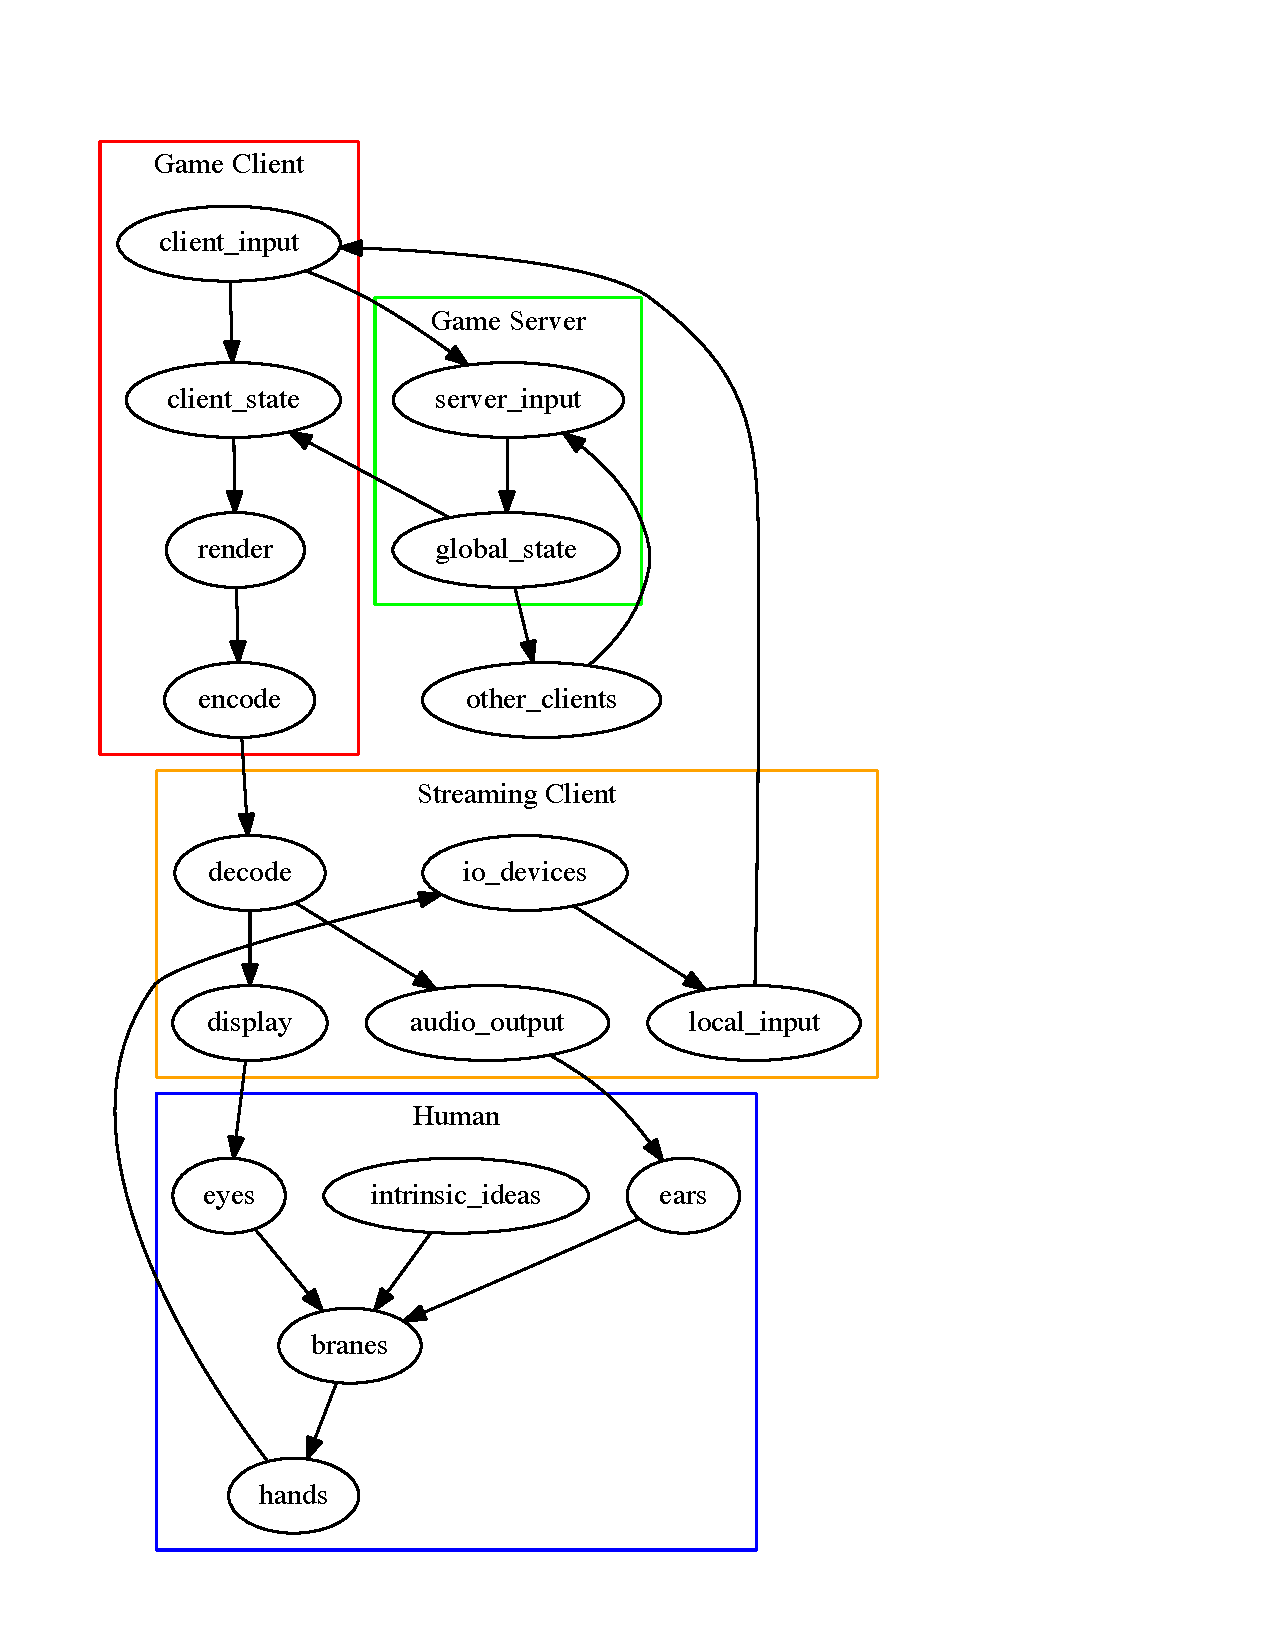
\includegraphics[width=1.0\columnwidth]{../models/cycle.pdf}
  \caption{Interaction of TODO.}
  \label{fig:component-model}
\end{figure}

At the end of this section, the reader should agree that end to end latency is a sensible starting point to study video game qos.


%%%%%%%%%%%%%%%%%%%%%%%%%%%%%%%%%%%%%%%%%%%%%%%%%%%%%%%%%%%%%%%%%%%%%%%%%%%%%%%%
\subsection{Measurement Approaches}
\label{sec:measurementapproaches}

With these metrics, test parameters, and categorizations in mind, one can now attempt to conduct the actual measurements of which there are three distinct methods each situated at a unique vantage point as depicted in Fig.~\ref{fig:measurement-methods}.

\begin{figure}[!t]
    \centering
    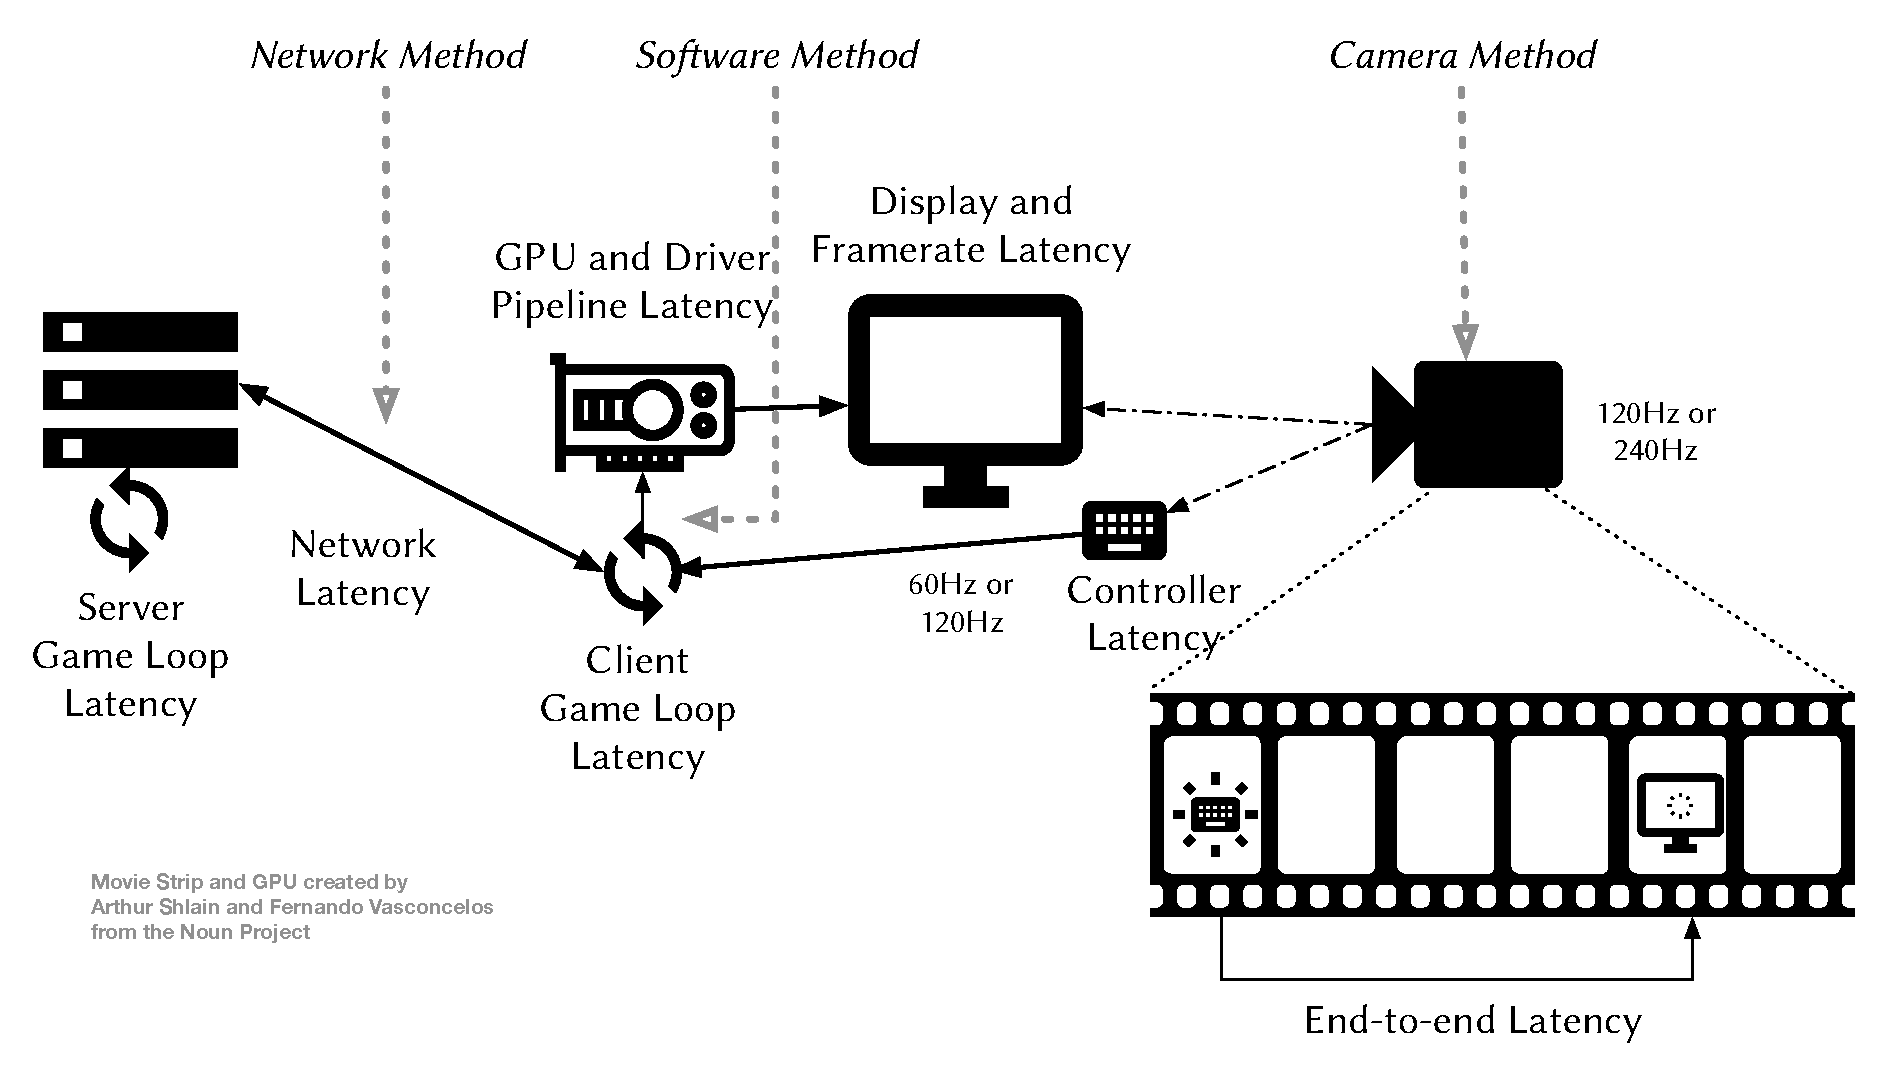
\includegraphics[width=1.0\columnwidth]{../models/e2e-lag.pdf}
    \caption{Location of the three measurement approaches to capture end-to-end latency inside a usual online video game lag chain.}
\label{fig:measurement-methods}
\end{figure}


%%%%%%%%%%%%%%%%%%%%%%%%%%%%%%%%%%%%%%%%%%%%%%%%%%%%%%%%%%%%%%%%%%%%%%%%%%%%%%%%
\subsubsection{Screen Recording Software Method}

Recording the output stream of a video game might be the simplest approach. It can capture both the framerate and \gls{IAT} at a driver level, and the recorded video can be used for image and quality analyses as well as to correlate it to additionally recorded input events to calculate the lag. This is not the the complete end-to-end lag however, as both the controller and screen output latency are missing. The need to install additional software might make it unsuitable for some scenarios, e.g., when measuring console video games. As a variant of this method, one can also record the output stream with a video capture card on a secondary computer, which does not negatively effect the game's performance as the software method does.

Examples of this approach include both \cite{Chen:2011:MLC:2072298.2071991} and \cite{6670099} which measured the end-to-end latency of cloud gaming services in the game client. They do this by invoking the system menu in games and measuring the time until it is displayed. A 2013 paper \cite{6574660} investigates the quality of cloud gaming interactiveness (i.e., the lag) as well as image quality by employing software recording methods on the client's computer.
%However, this method assumes a constant delay of game actions and may not capture the actual end-to-end lag of many of real game actions, as they are typically different from and longer as the latency of displaying a menu. A 2013 paper \cite{6574660} investigates the quality of cloud gaming interactiveness (latency) as well as image quality by employing software recording methods on the client's computer. With these techniques the challenges regarding the quality are discussed.


%%%%%%%%%%%%%%%%%%%%%%%%%%%%%%%%%%%%%%%%%%%%%%%%%%%%%%%%%%%%%%%%%%%%%%%%%%%%%%%%
\subsubsection{Passive Network Measurements}

In some cases it may also be advantageous to tap into the network interactions of the games and record the command and update messages sent between server and clients. While this is not a direct measure of game quality, it can give insights into the game's inner workings, such as the tick rates, and one can derive, e.g., the lowest achievable end-to-end lag from this.

%Can only investigate command and update messages, not tick rate directly. Evaluate rate, IAT, and bandwidth, estimate latency (though there may be no direct link between commands and updates).

Besides simple flow-based or packet-counting network metrics, many games also allow for deeper packet-dissecting analyses, as the often rely on standardized protocols or data formats, such as Protobuf\footnote{\url{https://developers.google.com/protocol-buffers/}} or incorporate well-known third-party multiplayer-enabling libraries. %And cloud games sometimes use derivates from the RTP-family or XMPP-based(VERIFY) protocols. 
Additionally, almost no game encrypts its time-critical messages, enabling an easy read-out. Through these means, the specific commands can be read from the network and potentially linked to their effect on the game state in the corresponding state update messages.
%, but also potentially allowing malicious actions to be taken easily.


%%%%%%%%%%%%%%%%%%%%%%%%%%%%%%%%%%%%%%%%%%%%%%%%%%%%%%%%%%%%%%%%%%%%%%%%%%%%%%%%
\subsubsection{Camera Recordings}

The only method to fully capture the end-to-end lag is to simultaneously record both the screen and input device through an external camera. The experimenter then has to count the frames between pressing a button on the input device and the action appearing on the screen and calculate the lag from this. For better visibility the input device is usually modified with an LED that turns on when the button is pressed. Also, the camera should operate at least at twice the monitor's refresh rate according to the Nyquist-Shannon sampling theorem. An additional benefit of this method is, that the game and the computers remain unaltered and are therefore not affecting any game mechanics. This approach is often used in the gaming press and by game developers to evaluate a game's control fidelity. A variant of this approach, replacing the camera with a photodiode and synthetically creating the input events with a microcontroller is described in \cite{beyermethod}, though it may be difficult to use for certain game actions that have a barely visible or unpredictable on-screen effect.

